% $Id$

\subsection{Program Organization}

The demonstration program consists of a top level Application
Driver, a top level Gridded Component, and nested within this Gridded
Component are 3 subcomponents: a Coupler Component and 2 Gridded Components.

The following diagram shows this organization.  Note that there
is no direct communication between the subcomponents; all
interactions are mediated by the top level Gridded Component.

Each component communicates via initialize, run, and finalize
subroutine calls.  These go through the ESMF library where
they are checked for validity, default values are supplied,
and only those components involved in the computation are
invoked.

% the bpht says we prefer the bottom of a page, then separate page,
% then here, then top last.

\begin{figure}[bpht]
\caption[Components]{Structure of the demonstration program.}
\label{fig:democomps}
\begin{center}
\scalebox{0.70}{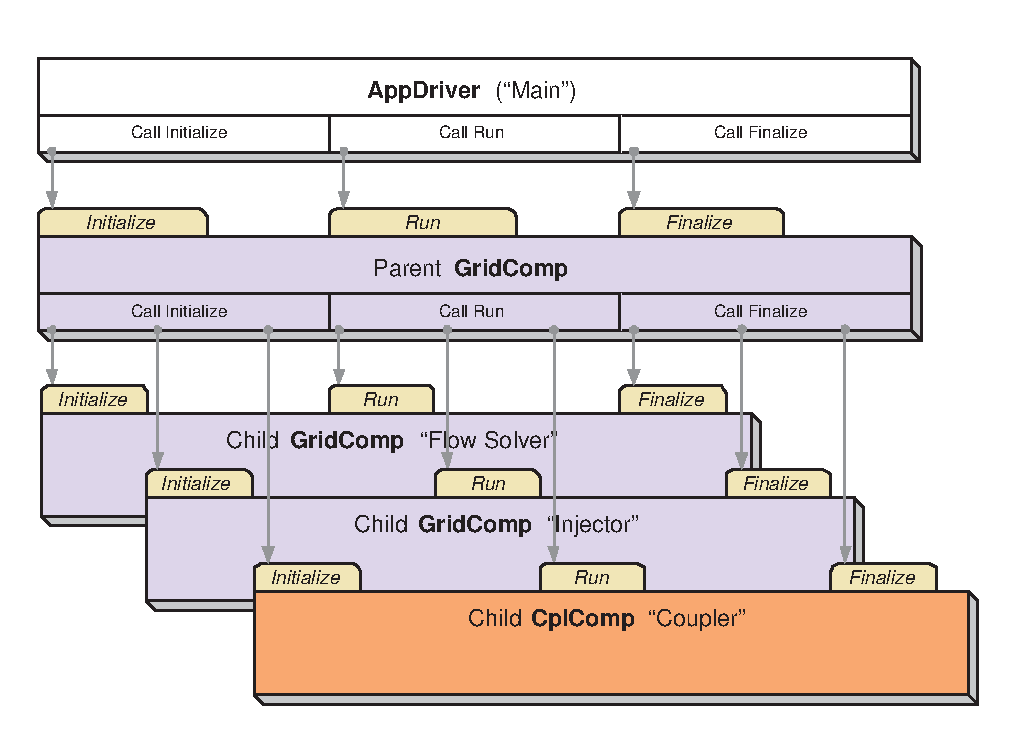
\includegraphics{flow_struct.eps}}
\end{center}
\end{figure}


